\documentclass{report}

\usepackage{ctex}
\usepackage[a5paper,top=0.8in,bottom=1in]{geometry}

\usepackage{amssymb}
\usepackage[version=4]{mhchem}
\usepackage{hyperref}

%\usepackage{setspace}
%\setstretch{1.23}

\usepackage{xcolor}
\definecolor{myblue}{rgb}{0.172,0.439,0.729}

\usepackage{marginnote}
\newcommand{\mnote}[1]{\marginnote{\footnotesize\textit{\textcolor{gray}{#1}}}[0ex]}
\newcommand{\fnote}[1]{\footnote{#1}}

\usepackage{natbib}
\setlength{\bibsep}{0.0pt}
\usepackage{astroabrev}
\bibpunct{(}{)}{;}{a}{}{,}

\usepackage{graphicx}
\renewcommand{\figurename}{图}
\newcommand{\reffig}[1]{图~\ref{#1}}
\newcommand{\refstep}[1]{第~\ref{#1}~步}

\newcommand{\mitem}{$-$~}

\usepackage[inline]{enumitem}

\usepackage{xeCJK}
\setCJKmainfont[BoldFont=STHeiti, ItalicFont=Kaiti SC Bold]{STSong}
\setCJKsansfont[BoldFont=STHeiti]{STXihei}
\setCJKmonofont{STFangsong}

\usepackage{fontspec}
%\setmainfont[Ligatures=TeX]{Georgia}
%\setsansfont[Ligatures=TeX]{Arial}

\usepackage{titlesec}
\titleformat{\chapter}[block]{\huge}{\textbf{第\chinese{chapter}章}}{1ex}{\textbf}
%\titleformat{\section}[block]{\Large}{\chinese{section}.}{1ex}{}
%\titleformat{\subsection}[block]{\large}{\arabic{subsection}.}{1ex}{}
%\titleformat{\subsubsection}[block]{}{(\arabic{subsubsection})}{1ex}{}

%宇宙有机物分布与生命起源
%
%1. 引言
%1.1 毫米波分子天文学简史
%1.2 往亚毫米波段扩展的必要性
%
%2. 星际有机物和生命分子
%2.1 复杂有机分子的发现
%这一节是综述,讲已发现的各种分子,特别是有机分子。会讲观测手段、观测的源的特性,等等。
%2.2 复杂有机分子与生命分子的关联
%这一节带有推测性,把话题从分子天文导向天体生物 (astrobiology),讲天文观测、特别是对复杂有机分子的观测对认识生命起源的意义。
%2.3 使用60米望远镜探测有机分子、生命前分子、生命分子的前景
%这一节比较具体和实在,从技术细节的角度讲60米望远镜能在探测有机分子、生命前分子、生命分子方面做什么,会讨论不同的观测策略 (不同的科学目标有不同的观测策略)、预期观测的源的类型和/或覆盖的天区、达到什么样的观测深度、得到什么样的结果。这里并没有预设只观测特定类型的源 (比如Sgr B2或者IRAS16293那样的),完全可以把行星状星云、超新星遗迹等类型的源包含进来,也没有预设只做无偏巡天。
%这一节篇幅可能会显著长于其它节,有必要的话可以再拆分,写出来了再说,现在还没写。
%2.4 星际分子到行星系统的迁移
%这一节讲物质从星际空间转移到行星系统的过程,其实主要就是讲原行星盘,包括在原行星盘里探测复杂分子的可能性,或者就算不能 —— 对原行星盘的研究能对厘清“星际物质-星周物质-生命起源”这个逻辑链条做出哪些贡献,以及60米望远镜能做些什么 (比如通过巡天能力提高样本数以供后续研究)。
%2.5
%星际物质与太阳系内天体物质构成的关系
%接上一节,太阳系 (our solar system) 这样的行星系统的物质终究是来自原行星盘的气体和尘埃,那么对太阳系内天体的研究可以为“星际物质-星周物质-生命起源”这个链条提供更多佐证;对其它行星的观测也可以为认识地球环境的特殊性提供对比。这里会讨论60米望远镜能不能对太阳系内天体的观测做出贡献 (如果不能,就删掉这节)。
%
%3. 宇宙中的有机物分布
%3.1 近邻星系中的有机物分布
%3.2 更远星系中的物质组成


\newcommand\refeq[1]{(\ref{#1})}

\newcommand\Hii{H\;\textsc{ii}}
\newcommand\irassixteen{IRAS\;16293-2422}
\newcommand\sgrb{Sagitarius B2}
\newcommand\twh{TW Hydrae}

\title{大型亚毫米波观测设备\\%
项目建议书}
\author{}

\begin{document}

\maketitle

\chapter{宇宙有机物分布与生命起源}
%\author{60 米级亚毫米波望远镜“宇宙物质与生命起源”工作组}

%\section{分子天文学的兴起和发展}

有两个问题由来已久:
\begin{enumerate*}[label=\arabic*)]
  \item 地球上的生命如何起源?
  \item 地球之外是否存在生物、甚至智慧生命\footnote{这里“生物”一词包括从病毒、细菌等微生物一直到哺乳动物等,而“智慧生命”特指像人类一样已经发展出高度文明的生物。}?
\end{enumerate*}  
现代科学正在逐渐对这两个问题给出答案。

1952年的\href{https://en.wikipedia.org/wiki/Miller%E2%80%93Urey_experiment}{米勒-尤里实验}%
表明,在合适的物理条件下,可以通过简单无机分子的混合物合成多种复杂的生命分子 (氨基酸分子)。这表明从无机物到生命物质之间不存在不可逾越的鸿沟。

迄今已在星际空间探测到\href{http://www.astro.uni-koeln.de/cdms/molecules}{超过两百种}不同的分子,其中大部分是有机分子。天文界一般称包含原子数不少于六的分子为“复杂分子”;在星际空间探测到的复杂分子已超过70种,其中的一些分子与生命的产生有密切关系。另外,与地球生命密切相关的分子,包括水、氧气、二氧化碳等分子也都已在星际空间探测到。

这些发现提示我们: \begin{enumerate*}[label=\arabic*)]\item 生命物质很可能在宇宙中普遍存在,\item 地球生命的起源可以追溯到星际空间。\end{enumerate*} 如果顺着这样的推理更进一步,那么可以猜测:地球外有可能存在生命甚至智慧生命。探索生命起源和地外生命乃至地外文明有助于认识人类和地球在宇宙中的地位,可以为人类文明的远期发展提供指导。不妨做一个历史的类比:数百年前欧洲人通过大航海发现了新大陆,以此奠定今天的世界格局;由于地球资源有限,未来的人类若要持续发展,前往太空是一个可能性很大的选择,因此对星际空间物质组成的探索至关重要。

大型亚毫米波望远镜可以极大地推动关于星际分子的研究,为认识生命的星际空间起源提供事实依据。我们提议对不同类型的天体,分层次进行观测:通过大规模巡天认识银河系的大尺度有机物分布,通过在星际空间搜寻生命前分子和生命分子为生命在星系尺度上的广域分布提供线索,通过对原行星盘、残盘、以及正在形成过程中的行星系统的观测认识物质从星际介质到行星系统的转移过程,通过对太阳系天体的观测认识太阳系物质的星际起源,最后,还可在宇宙尺度上探索复杂分子的分布。下面给出详述。

\section{银河系宽波段深度巡天}
%Wide band deep submillimeter survey of the Milky Way
%WBDSSMW
%DSS

在毫米波和亚毫米波段存在丰富的分子谱线。对于典型的星际物理环境,分子转动跃迁谱线发射的峰值出现在这个波段内。因此,在这个波段内的宽波段深度谱线巡天可以发现大量的分子,提供独一无二的银河系内分子物质、特别是有机物质的分布地图,同时为认识银河系的全局结构、物理状态、演化提供重要数据。

目前已经有一些正在进行或已经完成的巡天项目,下面选择有代表性的几个简单介绍,为新巡天项目提供参考:
\begin{description}
  \item[银河画卷巡天] 这是基于紫金山天文台青海观测站13.7米望远镜及配备的多波束超导成像频谱仪的巡天项目 \citep{Lu2018},对银河系$-10^\circ\le l\le 250^\circ$, $|b|\le5^\circ$区域进行\ce{$^{12}$CO}, \ce{$^{13}$CO}, \ce{C$^{18}$O}的 $J=1{-}0$ 转动跃迁观测,空间分辨率为$30''$,噪声水平达到 0.3 K。目前已大约完成全部巡天工作的一半,在银河系大尺度结构、恒星形成、超新星遗迹与分子云的相互作用等方面取得了较多成果。
  \item[WISH] WISH 是 Water In Star-forming regions with Herschel 的缩写,是Herschel空间望远镜 (已退役) 的一个关键项目,通过水和相关的分子研究年轻恒星体的化学结构以及水的丰度从塌缩云到原行星盘的演化,跨越了不同演化阶段和光度差异很大的不同天体。相关的巡天项目包括CHESS (Chemical HErschel Surveys of Star forming regions, 恒星形成区的化学) \citep{Ceccarelli2010}, HEXOS (Herschel observations of EXtra-Ordinary Sources, 研究Orion PDR的化学) \citep{Bergin2010}, SOLIS (Seeds Of Life In Space, 使用IRAM-NOEMA研究处于不同环境和演化阶段的中低质量恒星形成区的关键有机分子) \citep{Ceccarelli2017}, 等等。
\end{description}  
本巡天项目会在频谱覆盖范围、频谱分辨率、灵敏度、空间分辨率、空间覆盖范围等方面全方位超过类似的巡天项目。根据已有的观测结果和理论外推,同时考虑到望远镜的预期技术指标和观测的现实可行性,提出以下巡天参数:
\begin{itemize}
  \item 频率覆盖范围: 75 GHz -- 260 GHz
  \item 频谱分辨率: 100 kHz (高频段这个值可能会大一些)
  \item 灵敏度 (噪声水平): 10 mK
  \item 空间分辨率: 7$''$ (@260 GHz) -- 17$''$ (@75 GHz)
  \item 空间覆盖范围: $-10^\circ\le l\le 250^\circ$, $|b|\le5^\circ$
\end{itemize}  
需要的总观测时间可通过下式估计
\begin{equation}
\begin{split}
  t_\text{total} \simeq
  & \left(\text{一天}\right) \times\\
  & \left(\frac{\text{总面积}}{\text{视场面积}}\right)\times \\
  & \left(\frac{\text{频率范围}}{\text{瞬时带宽}}\right)\times \\
  & \left(\frac{\text{频谱分辨率}}{100\;\text{kHz}}\right)^{-1}\times \\
  & \left(\frac{1\;\text{mK}}{\text{灵敏度}}\right)^2\times \\
  & \left(\frac{T_\text{sys}}{100\;\text{K}}\right)^2
\end{split} 
\end{equation} 
使用计划中的多波束宽带接收机 (视场1度,带宽16 GHz),完成这个巡天项目大约需要1年的对源观测时间。初期多波束也许不能一次全部上线,因此可以先对重点区域在部分频段进行巡测。下面依次描述重点关注的天文对象。
%\subsection{氢电离区 (\Hii{} region)}
\subsection{光致离解区} 即远紫外光子主导气体的能量平衡和化学的区域 \citep{Tielens2005} ,简称 PDR,photodissociation region, 也叫光子主导区, photon-dominated region。PDR区是合成星际复杂有机分子的重要场所。尘埃表⾯冰物质中的多环芳香烃 (PAH) 的氢原子可以在紫外辐照下被各种功能基团 (如OH,\ce{CH3},COOH,\ce{NH2},\ce{OCH3},CN,CO 等)取代,形成 太阳系天体所具有的复杂有机物 \citep{Bernstein2002},包括各种氨基酸 \citep{Bernstein2002a}。如果这种机制确实在分布 范围极广的各类PDR区域发挥作用,其产生的复杂有机物的产量和种类可以非常可观,从⽽成为地球生 命起源的重要有机物来源。

几个典型的PDR区域包括猎户座马头星云、猎户座Orion bar、Mon R2等,它们的远紫外辐射场强度不同,化学成分也有差异。较弱的远紫外光子可以把尘埃表面凝结的复杂有机分子解吸附到气态从而可被观测到,而强的远紫外光子会把气态的复杂有机分子和多环芳香烃击碎,变成简单有机分子。由于尘埃和气体的消光作用,不同深度处的远紫外辐射场强度不同,导致PDR区域的化学成分呈分层结构,不同的分子出现在不同层面。在这些PDR里已经探测到丰富的有机分子,包括\ce{C2H}、\ce{C4H}、\ce{c-C3H2}、\ce{c-C3H}、\ce{H2CO}、\ce{CH3OH}、\ce{H2CCO}、\ce{CH3CHO}、\ce{H2CS}、\ce{HCOOH}、\ce{CH3CN}、\ce{CH2NH}、\ce{HNCO}、\ce{HC3N},\ce{CH3C2H},等等。行星状星云、原行星盘的部分区域也可能进行着类似于 PDR 的光化学反应过程。

对整个银河系中远紫外光子驱动复杂有机物形成的情况还很不清楚,需要更加系统全面的 巡天观测加以确定。
%O、B型年轻恒星发出的极强UV辐射照射到近邻分子云表面,由于尘埃和气体消光,在分子云表面形成从原子离子到内部中性分子的层状化学分布。

\subsection{热分子云核 (hot core, hot corino)}
热分子云核是被正在形成的原恒星加热的致密热尘埃气体云的核心部分,通常尺度小于0.01{} pc,温度可达100 K以上。观测表明大质量热云核 (hot cores) 与小质量热云核 (hot corinos) 存在显著差异:后者的尺度、密度、温度都低于前者,但复杂有机分子相对\ce{CH3OH}的丰度比前者高一个量级以上 \citep{Caselli2012}。

热云核中的复杂有机分子的合成与尘埃表面化学反应密切相关。在恒星形成开始之前的冷云核阶段,尘埃颗粒表面的冰层可能就因宇宙射线诱导的FUV光致离解反应已经产生并保存了相当可观的复杂自由基 (如HCO, \ce{CH3O}等),然后在热云核塌缩升温阶段被蒸发到气相然后反应生成复杂有机分子 (如\ce{H2CO}, \ce{CH3OH}, \ce{HCOOH}, \ce{HCOOCH3}, \ce{CH3OCH3}等),丰度可达$10^{-9}-10^{-7}$。在此基础上,\citet{Garrod2008}认为云核塌缩升温的时标越长,越有利于形成更多的复杂有机分子,比如含羟基 (OH) 的 \ce{CH3OOH}, \ce{CH2(OH)2}, \ce{HOCOOH},酰胺类物质 (amide) 的\ce{NH2COOH}和\ce{(NH2)2CO},以及含氨基 (\ce{NH2}) 的\ce{CH3ONH2},\ce{CH2OHNH2}, \ce{NH2OH}等。

距离我们最近的大质量恒星形成区中的一个热云核是位于猎户座-麒麟座分子云复合体中的OMC-1 (也称 Orion-KL)。这个区域具有复杂的化学和动力学结构。通过从70 GHz到903 GHz的宽波段谱线观测已经在这个源的近邻探测到超过20种复杂有机分子,不同类型的分子 (比如含氮或者含氧的复杂有机分子) 具有不同的分布。

\irassixteen 是小质量恒星形成区小热云核的一个著名例子。这个源是一个双星结构,其中一个核有丰富的含氧复杂有机分子发射,而另一个则以较简单的含氮和含硫分子为主。一些复杂有机分子既出现在热云核中,也出现在周围延展的冷气体中,而长碳链分子仅出现在冷气体中。高空间分辨率频谱巡天探测到了 10000 多条谱线,认证出了乙醇醛 (\ce{CH2OHCHO})、甲酸甲酯 (\ce{HCOOCH3})、乙酸 (\ce{CH3COOH}),以及乙二醇 (\ce{(CH2OH)2}) 的同分异构体等复杂分子。分子云他所阶段低温尘埃表面化学反应对这些生命前分子合成至关重要。

这些热分子云核里形成的复杂有机分子到达行星的途径包括:在恒星形成过程中流向星周吸积盘,然后在行星的形成过程中被吸积到行星上,或者凝聚到尘埃表面然后通过彗星、流星、陨石等载体到达行星。这些复杂有机分子会成为行星上生命物质的原材料。热云核里的分子也会被吸积到正在形成的恒星里,或者被恒星的辐射压或星风驱散到星际空间。对各种复杂有机分子的演化路径的研究是一个重要课题。

\subsection{冷暗分子云}
\subsection{年老恒星周边}
\subsection{超新星遗迹}

\section{搜寻生命前分子和生命分子}

氨基酸、糖类、酯类\footnote{“酯”对应的英文是ester,指的是醇与羧酸或无机含氧酸发生酯化反应生成的产物。“脂”对应的英文是lipid,是脂肪酸与醇脱水缩合生成的酯及其衍生物的统称,其中包括脂肪、蜡、类固醇、脂溶性维生素、单酸甘油酯、二酸甘油酯、磷脂等 (参考: \url{https://en.wikipedia.org/wiki/Lipid}%
)。按照这些描述,酯是脂的子集。从天文可探测性的角度考虑,下文仅讨论较简单的酯类。}、核苷酸等分子是构建生命体和维持生命运转和演化的基本物质,可被称为生命物质,而形成这些大分子的前体物质可被称为生命前分子。这些生命前分子和生命分子在星际空间的存在性对于生命起源问题的研究至关重要。最简单的糖类、酯类分子分子已经在星际空间被探测到,比如乙醇醛 (\ce{HOCH2CHO})\footnote{单糖的化学式为\ce{(C\cdot H2O)$_n$}, $n\ge3$,而乙醇醛对应的$n$是2,所以严格地讲乙醇醛不属于糖类。}\citep{Hollis2000,Jorgensen2012},甲酸甲酯 (\ce{HCOOCH3}) \citep{Sakai2006}, 甲酸乙酯 (\ce{HCOOCH2CH3}) \citep{Belloche2009}, 乙酸甲酯 (\ce{CH3COOCH3}) \citep{Tercero2013} 等。

\subsection{寻找氨基酸}
已经在陨石中探测到几十种氨基酸 (超过地球生命自然含有的氨基酸种类数) \citep{Kvenvolden1970,Schmitt2010},彗星的彗尾中也探测到了甘氨酸 \citep{Altwegg2016};考虑到陨石和彗星的可能的星际起源,可以推测星际空间很可能存在氨基酸。

\citet{Garrod2013} 和 \citet{Suzuki2018}基于化学模型计算对甘氨酸分子 (glycine) 的丰度做出了预测。在合适的物理条件下,其丰度相对氢可达$10^{-10}$。基于比较乐观的物理条件,\reffig{figGlycine}给出了计算出的甘氨酸分子的发射谱线。可以看出在$\sim$110--150 GHz频段内具有较高强度,可达 5 mK。假定 100 K的系统噪声温度和100 kHz的频谱分辨率,可以通过大约10小时的积分达到$3\sigma$的探测。

如果能在星际空间直接探测到氨基酸分子,意味着生命物质的演化可以追溯到行星形成之前,对生命的起源和分布的研究也许将会变成一个天文问题。

\begin{figure}[htbp]
\centering
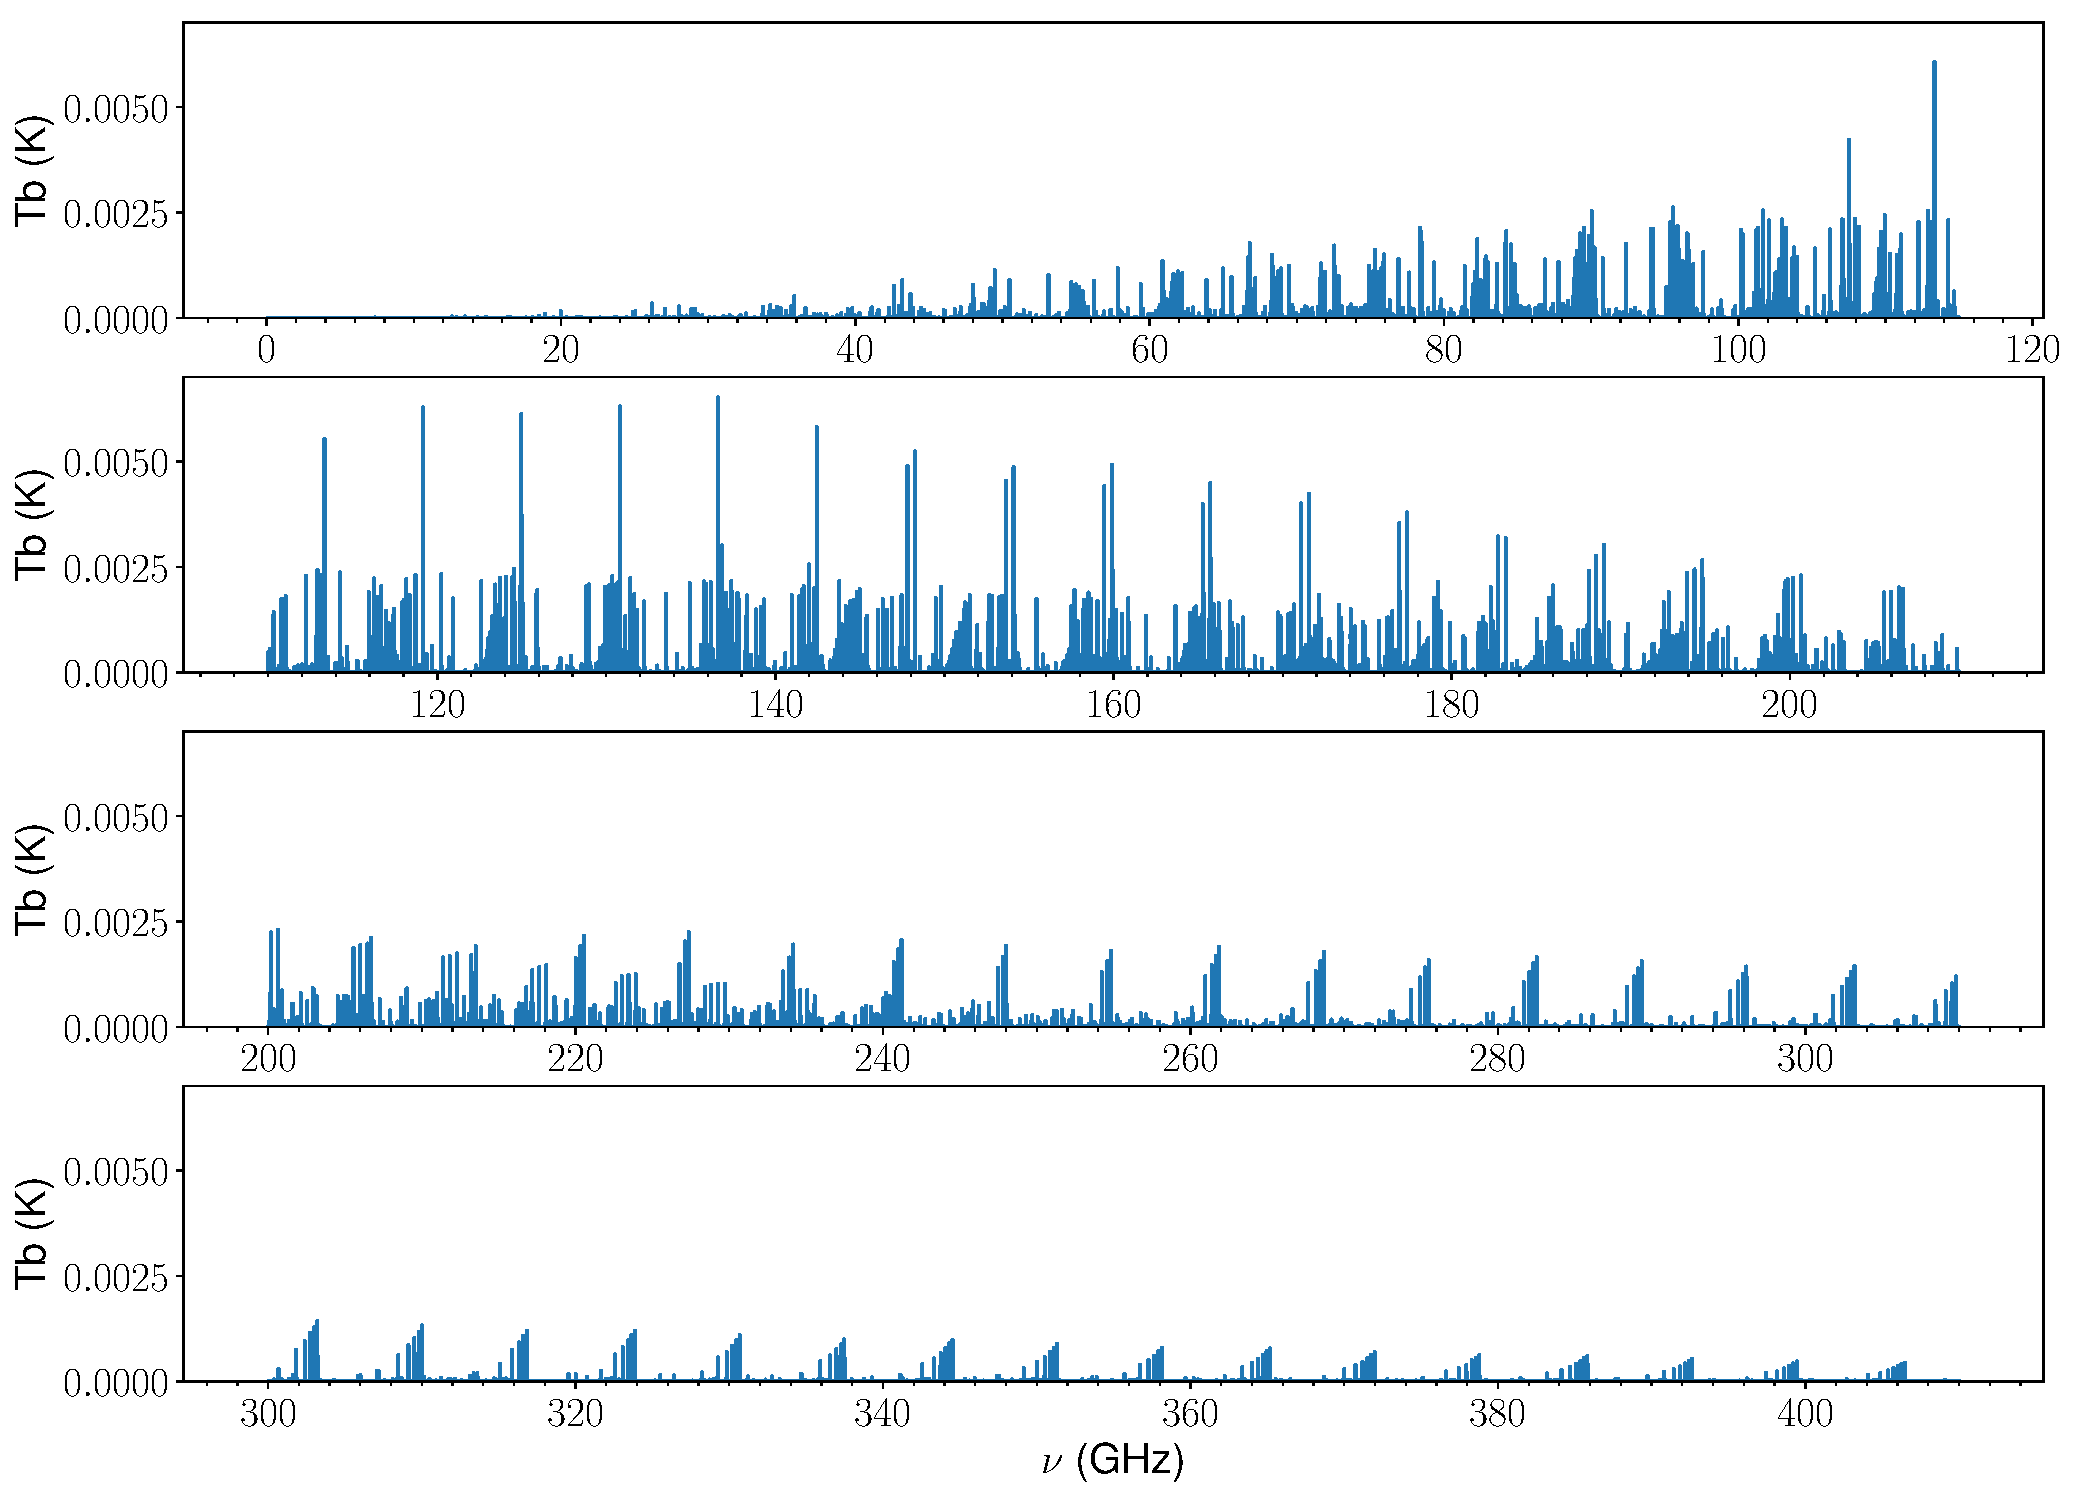
\includegraphics[width=0.95\linewidth]{glycine_50K_1e13_10e5_2e5.pdf}
\caption{计算出的甘氨酸从厘米波到亚毫米波的谱线,假定温度$T=50$ K, 柱密度$N_\text{glycine}=10^{13}$ cm$^{-2}$, 速度弥散$\delta V=2$ km s$^{-1}$。\label{figGlycine}}
\end{figure}

\subsection{糖类、酯类分子的探测}

糖类分子的通式为 \ce{C$_m$(H2O)$_n$} ($m$可以与$n$不同),单糖的通式是 \ce{(C\cdot H2O)$_n$} ($n\ge3$)。所以比已经探测到的乙醇醛略复杂的糖分子是 \ce{(CH2O)3},也就是甘油醛 (Glyceraldehyde),包含12个原子,迄今还没在星际介质中被探测到 \citep{Hollis2004}。通过实验室对星际冰类似物的研究表明甘油醛在星际尘埃冰壳里的存在性的可能性很大 \citep{deMarcellus2015},等待着被探测到。

酯类分子的通式为 \ce{RCOOR$'$},这里 \ce{R} 和 \ce{R$'$} 代表任何烷基 (\ce{C$_n$H$_{2n+1}$}) 或芳香基,R也可以是一个氢原子。可以看到,甲酸甲酯 (\ce{HCOOCH3}) 是最简单的酯类,复杂度略高的是甲酸乙酯 (ethyl formate) 和乙酸甲酯 (methyl acetate),含有11个原子,已在星际空间被探测到。更复杂的酯类分子的可探测性尚属未知。

\subsection{核苷酸 (nucleotide),核苷 (nucleoside),碱基 (nucleobase)}

这三者之间的关系是:
\begin{equation}
\begin{split}
\text{核苷酸} =&\, \text{核苷} + \text{磷酸基团}\\
\text{核苷}   =&\, \text{碱基} + \text{环状核糖或脱氧核糖}
\end{split} 
\end{equation}
% https://en.wikipedia.org/wiki/Nucleobase
核苷酸以一个含氮碱基作为核心,加上一个五碳糖和一个或者多个磷酸基团组成\footnote{\url{https://en.wikipedia.org/wiki/Nucleotide} \url{https://en.wikipedia.org/wiki/Nucleobase} \url{https://en.wikipedia.org/wiki/Nucleoside}}。这样的结构对于现在的星际分子探测手段而言还是太复杂了,
短期内应该不会被作为直接探测目标 (除非观测手段或者灵敏度能有重大突破)。

有五种碱基被称为基元碱基 (primary):腺嘌呤 (adenine, \ce{C5H5N5}, A), 鸟嘌呤 (guanine, \ce{C5H5N5O}, G), 胞嘧啶 (cytosine, \ce{C4H5N3O}, C), 胸腺嘧啶 (thymine, \ce{C5H6N2O2}, T), 尿嘧啶(uracil, \ce{C4H4N2O2}, U)。它们的功能是作为基因编码的基本单元,A、G、C、T位于DNA中,而A、G、C、U位于RNA中。已经在陨石中发现了多种碱基 \citep{Callahan2011},所以在星际空间存在碱基分子的可能性是可预期的;较简单的碱基分子 (比如尿嘧啶和胞嘧啶) 也许会被率先探测到。
% https://en.wikipedia.org/wiki/Nucleobase

\subsection{含磷分子}

已在星际空间探测到的含磷分子仅有6种 (CP, PN, PO, HCP, CCP, \ce{PH3});考虑到磷元素对生命的重要性 (三磷酸腺苷、DNA
、RNA的组成元素之一,也存在于细胞膜中),有必要对含磷分子增加更多关注。
%\citet{Jimenez2018}


%,也已经在彗星的彗尾中探测到甘氨酸及其前体物以及磷元素 \citep{Altwegg2016}。

\subsection{生命分子手征性的起源}

许多生命分子具有手征性,包括糖类、DNA和RNA中的核苷酸,以及构成蛋白质的氨基酸 \citep{McGuire2016}。地球上所有生物体的氨基酸都是左手性的。

\citet{McGuire2016a} 在\sgrb 中探测到了手性分子环氧丙烷 (\ce{CH3CHCH2O}) 的存在,虽然这个观测在原理上还不能探测到手征超出。未来通过高精度、完整偏振状态的测量可以测出手征超出 (如果存在的话)。

\subsection{生命相关分子 (水、氧气、二氧化碳) 的巡测}

这些分子的谱线会受到地球大气吸收的较大影响,可以通过观测它们的同位素分子作为代替;在宇宙尺度上可以通过红移让这些分子的谱线避开地球大气吸收。

在原行星盘较内的行星形成区域探测这些分子,有助于认识行星宜居性的起源。

\section{探索行星形成早期环境的化学组成}

原行星盘,\twh,近邻行星系统,debris disk

%\citet{Walsh2016}使用 ALMA 在\twh 里探测到了\ce{CH3OH} ,但实测丰度比模型预期低了两个量级。 \citet{Walsh2014}

\section{探索太阳系物质构成的星际起源}

行星大气、卫星大气、彗星成分

\section{近邻星系中的有机物分布}

迄今已经在河外星系探测到超过60种不同的分子。作为银河系宽波段深度巡天的扩展,可以对银河系附近的星系 (比如大小麦哲伦云、仙女座星系 (M31)、M82等) 进行类似深度的巡天。
% https://en.wikipedia.org/wiki/List_of_nearest_galaxies
% http://www.astro.uni-koeln.de/cdms/molecules

\section{遥远星系中的物质组成}

来自遥远星系的光是在宇宙还很年轻的时候发出的,一般认为在那个时期宇宙的金属丰度还很低,因此不会形成复杂的有机分子。但宇宙早期第一代恒星的快速演化也许能形成较多碳、氮、氧等元素,在合适的物理条件下它们也许能形成复杂分子。对它们的探索可以作为望远镜的机遇性课题。

\section{小结:机遇与挑战}

\begin{itemize}
  \item
这样的深度巡天会产生大量数据。对这些数据的处理和诠释在计算能力和算法方面提出了挑战。需要自动化的谱线认证算法。
  \item
对新分子的探测需要完备而准确的谱线数据库,这需要通过实验测量获得。
  \item
新发现的分子多样性对化学模拟的预测能力和解释能力提出了更高要求。
\end{itemize}  



\bibliographystyle{apj}
\begingroup
\renewcommand{\section}[2]{}%
\bibliography{references}
\endgroup

\end{document}
